\subsection{Halterung}\label{sec: Halterung}
Das Konzept für die Halterung des CubeSats zielt darauf ab, eine effektive Lösung zu finden, um den CubeSat am Gyroskop zu befestigen. Dabei gilt es zu beachten, dass möglichst alle Seiten des CubeSats offen und zugänglich bleiben. Die Halterung soll an zwei Punkten mit dem Gyroskop befestigt werden. \\
\vspace{3mm}
Der Kern dieses Konzepts ist ein Käfigsystem, das aus zwei Hauptteilen besteht, nämlich einem Boden und einem Deckel. Dieses Design ist speziell darauf ausgelegt, den CubeSat vollständig zu umschließen und durch Schrauben sicher zu fixieren. Es gibt dann somit am Boden und am Deckel jeweils einen Verbindungspunkt zum Gyroskop.\\
\subsubsection{Boden}
\begin{figure}[H]
    \centering
    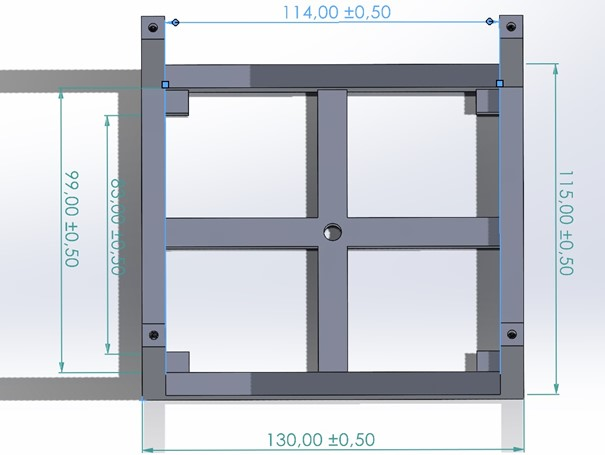
\includegraphics[scale = 0.5]{image/boden.jpg}
    \caption{Boden}
    \label{fig:enter-label}
\end{figure}
\vspace{3mm}
Das Bild zeigt eine technische Zeichnung einer rechteckigen Grundfläche mit den Maßen 130 mm in der Länge, 115 mm in der Breite und einer Materialstärke von 8 mm. Vier Pfosten erstrecken sich von den Ecken der Grundfläche, wobei die Pfostenlänge 77 mm beträgt.\\
\vspace{3mm}
In jedem Pfosten befindet sich eine Gewindebohrung, die eine Tiefe von 15 mm aufweist und für Schrauben mit einem Durchmesser von 4 mm vorgesehen ist. Im Mittelpunkt der Grundfläche ist ein Loch eingezeichnet, das als Befestigungspunkt für ein Gyroskop dient.\\
\vspace{3mm}
\begin{figure}[H]
    \centering
    \includegraphics[scale=0.7]{image/zusätzlichehalterung.jpg}
    \caption{Zusätzliche Halterung }
    \label{fig:enter-label}
\end{figure}
\vspace{3mm}
Jede Ecke der Struktur wird verstärkt, indem an jeder Ecke zwei zusätzliche Stützen angebracht werden. Diese Stützen dienen dazu, den CubeSat sicher und fest in der Struktur zu verankern, indem sie zusätzlichen Halt bieten und verhindern, dass sich der Satellit innerhalb des Trägerrahmens bewegt.\\
 \begin{figure}
     \centering
     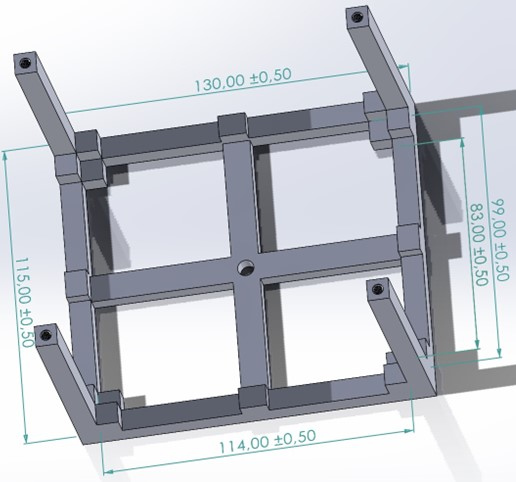
\includegraphics[scale=0.5]{image/fertiger boden.jpg}
     \caption{fertiger Boden}
     \label{fig:enter-label}
 \end{figure}

Um einen noch besseren Halt des CubeSats sicherzustellen, habe ich weitere Stützen jeweils in der Mitte der Grundfläche angebracht. Diese spannen den CubeSat noch besser ein und bieten dadurch eine noch bessere Stabilität.\\

\subsubsection{Deckel}
\begin{figure}[H]
    \centering
    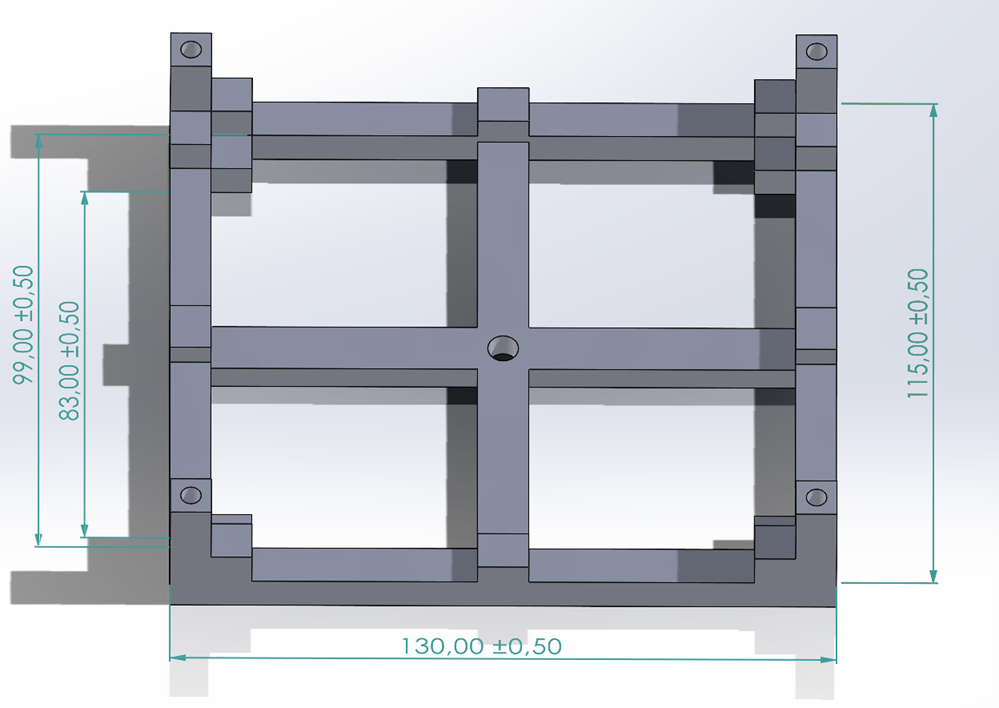
\includegraphics[scale=0.7]{image/deckel.png}
    \caption{Deckel}
    \label{fig:enter-label}
\end{figure}
\vspace{3mm}
Das Bild zeigt die technische Zeichnung einer rechteckigen Grundfläche, welche in seinen Grundmaßen und Konstruktionsmerkmalen dem Bodenteil ähnelt.\\
\vspace{3mm}
Die Abmessungen des Rechtecks betragen 130 mm in der Länge und 115 mm in der Breite, mit einer Toleranz von ±0,50 mm, und die Materialdicke ist ebenfalls gleichbleibend. Auch der Deckel hat im Mittelpunkt ein Loch, welches als Verbindung zum Gyroskop dient.\\
\vspace{3mm}
Der wesentliche Unterschied zwischen dem Deckel und dem Boden des Geräts besteht in der Länge der Pfosten, die beim Deckel auf 23 mm reduziert wurde, um eine Verbindung mit dem Boden mittels 4 cm langen Schrauben zu ermöglichen. Diese Anpassung sorgt für eine sichere Befestigung zwischen beiden Teilen.\\
\vspace{3mm}
Ein weiteres wichtiges Detail ist die Art der Löcher in den Pfosten. Während die Pfosten des Bodens Gewindebohrungen mit einer Tiefe von 15 mm aufweisen, die für Schraubverbindungen vorgesehen sind, sind die Pfosten des Deckels mit durchgehenden Löchern versehen. \\ 
\vspace{3mm}
Diese durchgehenden Löcher erlauben es, Befestigungselemente komplett durch die Pfosten hindurchzuführen, was eine durchgängige Verbindung zwischen dem Deckel und dem Boden aufweist.
\newpage
\subsubsection{3D-Druck der Halterung}
\begin{figure}[H]
    \centering
    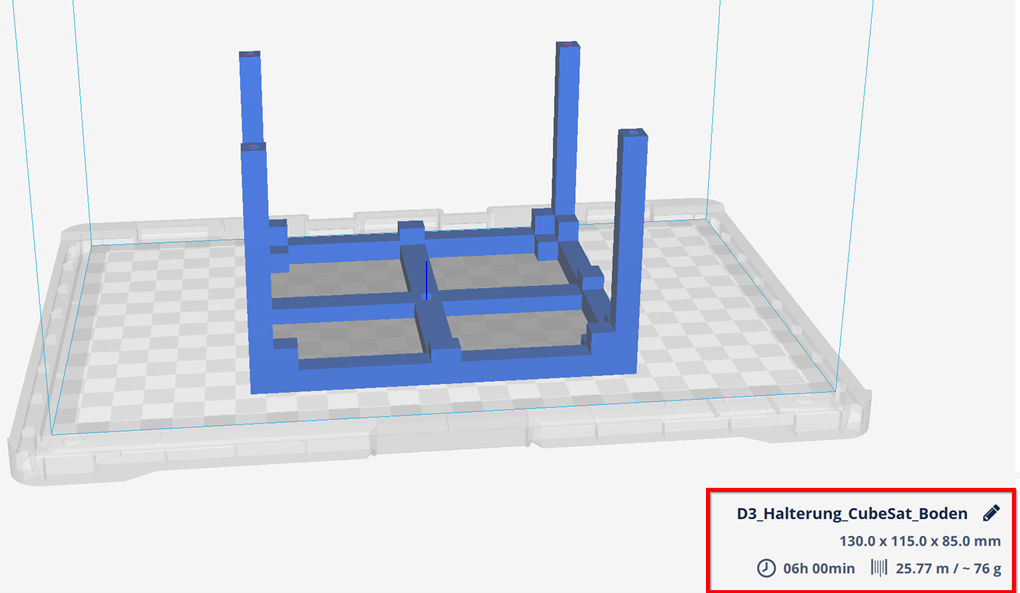
\includegraphics[scale=0.7]{image/druckvorbereitungboden.png}
    \caption{Druckvorbereitung für den Boden}
    \label{fig:enter-label}
\end{figure}
\vspace{3mm}
Abbildung zeigt, wie lange der Druckvorgang geht, wie viele Meter Filament benötigt wird und wie viel der Druck wiegt. Dieser Vorgang muss für den Deckel wiederholt werden.\\
\vspace{3mm}
\begin{figure}[H]
    \centering
    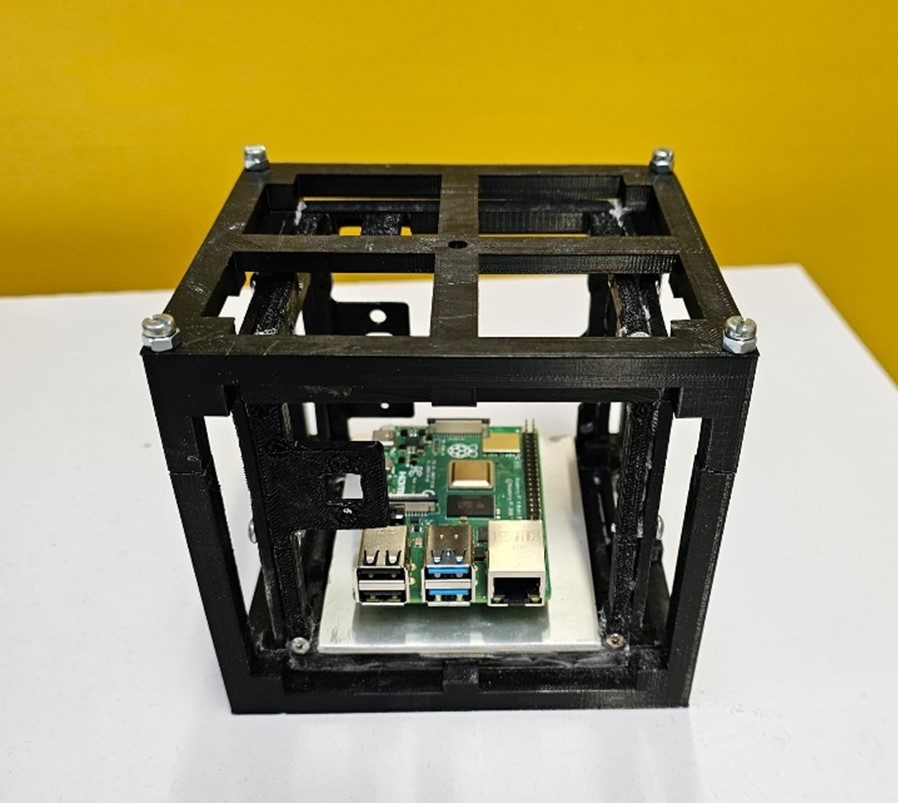
\includegraphics[scale=0.7]{image/cubeinhalterung.jpg}
    \caption{CubeSat in der Halterung}
    \label{fig:enter-label}
\end{figure}
\vspace{3mm}
Der CubeSat ist sicher im Käfig verankert. Der Käfig selbst besteht aus einer Struktur, die mit Schrauben und Muttern an den Ecken zusammengehalten wird. Die Konstruktion ist stabil und robust, was für eine gute Haltbarkeit spricht und somit bestens für die Rotationstests im Gyroskop geeignet ist. \\
\vspace{3mm}
\begin{table}[H]
    \centering
    \begin{tabular}{ | c | c | } 
  \hline
   \textbf{Bezeichnung} & \textbf{Stückzahl}\\ 
  \hline
   Schrauben  & 4\\ 
  \hline
  Muttern & 4 \\ 
  \hline
\end{tabular}
    \caption{Stückliste Halterung}
\end{table}